% Template for PLoS
% Version 3.5 March 2018
%
% % % % % % % % % % % % % % % % % % % % % %
%
% -- IMPORTANT NOTE
%
% This template contains comments intended 
% to minimize problems and delays during our production 
% process. Please follow the template instructions
% whenever possible.
%
% % % % % % % % % % % % % % % % % % % % % % % 
%
% Once your paper is accepted for publication, 
% PLEASE REMOVE ALL TRACKED CHANGES in this file 
% and leave only the final text of your manuscript. 
% PLOS recommends the use of latexdiff to track changes during review, as this will help to maintain a clean tex file.
% Visit https://www.ctan.org/pkg/latexdiff?lang=en for info or contact us at latex@plos.org.
%
%
% There are no restrictions on package use within the LaTeX files except that 
% no packages listed in the template may be deleted.
%
% Please do not include colors or graphics in the text.
%
% The manuscript LaTeX source should be contained within a single file (do not use \input, \externaldocument, or similar commands).
%
% % % % % % % % % % % % % % % % % % % % % % %
%
% -- FIGURES AND TABLES
%
% Please include tables/figure captions directly after the paragraph where they are first cited in the text.
%
% DO NOT INCLUDE GRAPHICS IN YOUR MANUSCRIPT
% - Figures should be uploaded separately from your manuscript file. 
% - Figures generated using LaTeX should be extracted and removed from the PDF before submission. 
% - Figures containing multiple panels/subfigures must be combined into one image file before submission.
% For figure citations, please use "Fig" instead of "Figure".
% See http://journals.plos.org/plosone/s/figures for PLOS figure guidelines.
%
% Tables should be cell-based and may not contain:
% - spacing/line breaks within cells to alter layout or alignment
% - do not nest tabular environments (no tabular environments within tabular environments)
% - no graphics or colored text (cell background color/shading OK)
% See http://journals.plos.org/plosone/s/tables for table guidelines.
%
% For tables that exceed the width of the text column, use the adjustwidth environment as illustrated in the example table in text below.
%
% % % % % % % % % % % % % % % % % % % % % % % %
%
% -- EQUATIONS, MATH SYMBOLS, SUBSCRIPTS, AND SUPERSCRIPTS
%
% IMPORTANT
% Below are a few tips to help format your equations and other special characters according to our specifications. For more tips to help reduce the possibility of formatting errors during conversion, please see our LaTeX guidelines at http://journals.plos.org/plosone/s/latex
%
% For inline equations, please be sure to include all portions of an equation in the math environment.  For example, x$^2$ is incorrect; this should be formatted as $x^2$ (or $\mathrm{x}^2$ if the romanized font is desired).
%
% Do not include text that is not math in the math environment. For example, CO2 should be written as CO\textsubscript{2} instead of CO$_2$.
%
% Please add line breaks to long display equations when possible in order to fit size of the column. 
%
% For inline equations, please do not include punctuation (commas, etc) within the math environment unless this is part of the equation.
%
% When adding superscript or subscripts outside of brackets/braces, please group using {}.  For example, change "[U(D,E,\gamma)]^2" to "{[U(D,E,\gamma)]}^2". 
%
% Do not use \cal for caligraphic font.  Instead, use \mathcal{}
%
% % % % % % % % % % % % % % % % % % % % % % % % 
%
% Please contact latex@plos.org with any questions.
%
% % % % % % % % % % % % % % % % % % % % % % % %

\documentclass[10pt,letterpaper]{article}
\usepackage[top=0.85in,left=2.75in,footskip=0.75in]{geometry}

% amsmath and amssymb packages, useful for mathematical formulas and symbols
\usepackage{amsmath,amssymb}

% Use adjustwidth environment to exceed column width (see example table in text)
\usepackage{changepage}

% Use Unicode characters when possible
\usepackage[utf8x]{inputenc}

% textcomp package and marvosym package for additional characters
\usepackage{textcomp,marvosym}

% cite package, to clean up citations in the main text. Do not remove.
\usepackage{cite}

% Use nameref to cite supporting information files (see Supporting Information section for more info)
\usepackage{nameref,hyperref}

% line numbers
\usepackage[right]{lineno}

% ligatures disabled
\usepackage{microtype}
\DisableLigatures[f]{encoding = *, family = * }

% color can be used to apply background shading to table cells only
\usepackage[table]{xcolor}

% array package and thick rules for tables
\usepackage{array}

% create "+" rule type for thick vertical lines
\newcolumntype{+}{!{\vrule width 2pt}}

% create \thickcline for thick horizontal lines of variable length
\newlength\savedwidth
\newcommand\thickcline[1]{%
  \noalign{\global\savedwidth\arrayrulewidth\global\arrayrulewidth 2pt}%
  \cline{#1}%
  \noalign{\vskip\arrayrulewidth}%
  \noalign{\global\arrayrulewidth\savedwidth}%
}

% \thickhline command for thick horizontal lines that span the table
\newcommand\thickhline{\noalign{\global\savedwidth\arrayrulewidth\global\arrayrulewidth 2pt}%
\hline
\noalign{\global\arrayrulewidth\savedwidth}}


% Remove comment for double spacing
%\usepackage{setspace} 
%\doublespacing

% Text layout
\raggedright
\setlength{\parindent}{0.5cm}
\textwidth 5.25in 
\textheight 8.75in

% Bold the 'Figure #' in the caption and separate it from the title/caption with a period
% Captions will be left justified
\usepackage[aboveskip=1pt,labelfont=bf,labelsep=period,justification=raggedright,singlelinecheck=off]{caption}
\renewcommand{\figurename}{Fig}

% Use the PLoS provided BiBTeX style
\bibliographystyle{plos2015}

% Remove brackets from numbering in List of References
\makeatletter
\renewcommand{\@biblabel}[1]{\quad#1.}
\makeatother



% Header and Footer with logo
\usepackage{lastpage,fancyhdr,graphicx}
\usepackage{epstopdf}
%\pagestyle{myheadings}
\pagestyle{fancy}
\fancyhf{}
%\setlength{\headheight}{27.023pt}
%\lhead{
\includegraphics[width=2.0in]{PLOS-submission.eps}}
\rfoot{\thepage/\pageref{LastPage}}
\renewcommand{\headrulewidth}{0pt}
\renewcommand{\footrule}{\hrule height 2pt \vspace{2mm}}
\fancyheadoffset[L]{2.25in}
\fancyfootoffset[L]{2.25in}
\lfoot{\today}

%% Include all macros below

\newcommand{\lorem}{{\bf LOREM}}
\newcommand{\ipsum}{{\bf IPSUM}}

%% END MACROS SECTION












\begin{document}
\vspace*{0.35in}

% Title must be 250 characters or less.
% Please capitalize all terms in the title except conjunctions, prepositions, and articles.
\begin{flushleft}
{\Large
% \textbf\newline{The sonic instructor: a music biofeedback system for improving weightlifting technique}
\textbf\newline{The sonic instructor: a music-based biofeedback system for improving weightlifting technique}
}
\newline
% Insert author names, affiliations and corresponding author email (do not include titles, positions, or degrees).
\\
Valerio Lorenzoni\textsuperscript{1,*},
Jacob Staley\textsuperscript{2},
Kelsey Onderdijk\textsuperscript{1},
Marc Leman\textsuperscript{1}

\bigskip

\textbf{1} Institute for Psychoacoustics and Electronic Music (IPEM), Department of Musicology, Ghent University, Ghent, Belgium
\\
\textbf{2}  Internet technology and data science lab (IDLAB), Ghent University, Ghent, Belgium
%\\
%\textbf{3} Data analysis Department, Ghent University, Ghent, Belgium
\\

\bigskip



 %Use the asterisk to denote corresponding authorship and provide email address in note below.
* valerio.lorenzoni@ugent.be

\end{flushleft}
% Please keep the abstract below 300 words

\section*{Abstract}
% Learning or only improving?!?

Functional coumpounds movements as in weighlifting and powerlifting disciplines are becoming increasingly popular. The 

Crossfit and gymnastic exercising are becoming increasingly popular. Functional movement are the the base of such exercises and 

usually these kind of movement require specific technique for movement improvement and 


\section*{Introduction}

%Biofeedback is a technique that typically uses electronic equipment to provide a client with auditory signals, visual signals, or both regarding internal physiological events, both normal and abnormal (eg, heart rate, blood pressure, and level of muscle activity).17 During biofeedback for gait retraining, the client is provided with augmented information (eg, kinematics, kinetics, and electromyography) regarding physiological responses. Additionally, biofeedback provides clinicians with a useful tool for giving clients instructions on how to modify movement patterns. Thus, biofeedback complements the already present internal feedback (ie, visual, auditory, and proprioceptive feedback) and acts as a ?sixth sense.?18 Biofeedback typically is provided instantaneously to the learner (ie, in real time), whereas other methods of external feedback (eg, verbal and video feedback) are provided some time after the movement. More recently, a resurgence of interest in real-time feedback has developed because of the expansion of technology related to kinematic19 and kinetic14,16 biofeedback.


Biofeedbacks have been used for over fifty years in the domains of sports \cite{onate2001augmented} and motor rehabilitation \cite{tate2016real,isakov2007gait}. These are used to provide the subjects with information about physiological or biomechanical parameters that that would otherwise be unknown \cite{giggins2013biofeedback}. The main goal of such systems is to let the subject automatically improve the performances at subconscious level, without explicit instructions by a trainer or therapist.

Traditionally biofeedback are presented to the subject via visual displays , acoustic or vibrotactile feedback. Recent technological developments have opened the possibility to provide such bio-feedback in real-time during physical activity, this opened the possibility for using

A recent development in rehabilitation is exercising in a gaming or virtual reality (VR) environment, thus providing a novel form of immersive biofeedback.


In this paper we describe the design and validation process of a bio-mechanical biofeedback system for improving weightlifting movements.

Weightlifting is an ancient sport which appeared in the Olympic Games in Athens already in 1896. Weightlifting movements are becoming increasingly popular in the sport world, as new sports as Crossfit (founded in year 2000 by) combine elements of Olympic weight lifting with power lifting and other disciplines.
Although researchers have proven the benefits of such functional weightlifting movements \cite{smith2013crossfit}, clear knowledge of the exact technique is required in order to maximize movement efficency and minimize the chance of injuries.

In this work we focused on a specific movement called \emph{deadlift} which is one of the three discipline of power lifting movements but it is widely used in weightlifting training and rehabilitation practices.

According to the handbook of the powerlifting federation \cite{} a deadlift consists of grabbing a barbell from the floor with hands, then raising the weight by extending the knee, hips, and back while holding the arms downward. On completion of the lift, the knees must be locked in a straight position and the shoulders pulled back.
McCuigan \emph{et al.} investigated the kinematics of deadlift comparing different techniques: the sumo and conventional style deadlifts.
Due to the fact that the deadlift is a closed chain exercise, it is often used in the prevention of and rehabilitation after anterior cruciate ligament (ACL) reconstruction to improve strength of the muscular structures that surround the knee and hence dynamic stability of the joint 

However, a wrong technique during deadlift lift-off may predispose the spine and back musculature to an increased risk of injury \cite{granhed1987loads,cholewicki1991lumbar}. The exercise is often made unsafe by the lifter rounding his back and bending over too far at the hips just before lifting. Holding the bar away from your body instead of right against it is another way to injure your back. 
With the presented system we aim at providing a real-time feedback using auditory displays, i.e. sonification. The quantities being sonified and on which the participant gets feedback are the spine curvature and the barbell horizontal displacement, as these quantities are directly related to back loads and injuries.
Usually coaches spend time in the first phase to teach the right technique and provide feedbacks to the performers.
Having continuous feedback by a coach is not feasible while training in public gyms or at home. Therefore there is need to develop portable systems able to guide towards the right movement technique.

The use of sonification in weightlifting has been shown to increase average exertion of power compared to silent condition \cite{murgia2012using}. The work of Fritz \emph{et al.}  \cite{fritz2013musical} showed that music agency stimulated by sonification is able to decrease perceived exertion during workout, indicating that musical agency may actually facilitate physically strenuous activities. These results further indicated that the positive effect of music on perceived exertion cannot always be explained by an effect of diversion from proprioceptive feedback. The most typical strategy pertains to a goal-driven approach. This approach requires that the learner has an explicit representation of the target behavior, i.e., the goal. Sonification then functions as mere information carrier, allowing people to monitor their behavior, compare it to the target behavior, and adapt their behavior if required [2?4]. 



Recently, a promising alternative strategy is being explored, drawing upon basic principles from the reinforcement learning paradigm. Reinforcement learning is rooted in the idea that people act and behave so as to maximize outcome reward. Hence, when coupling a reward to a desired behavior, people are likely to exhibit this behavior spontaneously, without needing to be told explicitly what to do. In this context, music and sound are particularly relevant as they might be rich sources of reward and pleasure (for an in-depth discussion, see [1])


In the present experiment we developed a sonification strategy which exploits the positive effects of music of music. 
Several authors reported the positive effects of music in sports and physical activities. In particular, music was shown to distract from fatigue and discomfort (Bood, Nijssen, Van Der Kamp, \& Roerdink, 2013;Yamashita, Iwai, Akimoto, Sugawara, \& Kono, 2006), enhance work output (Edworthy \& Waring, 2006; Rendi, Szabo, \& Szab, 2008), increase arousal (Szabo, Balogh, Gaspar, Vaczi, \& Bosze, 2009; Karageorghis \& Priest, 2012; Karageorghis \& Terry, 2011), and boost mood states (Edworthy \& Waring, 2006; Shaulov \& Lufi, 2009).

As formulated in the theory of embodied music interaction \cite{Marc_EmbodiedMusic,godoy2010musical}, listening to music generates motor coordination-inducing schemes that respond to external sensory sources in such a way that it allows auditory-motor alignment and even prediction of musical events. 

We developed a system that uses music quality as reward, i.e. the correctness of the movement is rewarded by an improving of the audio quality of the feedback. More specifically in this specific case the unwanted movements: spine forward bending and barbell forward displacement with respect to initial position are mapped ,respectively into: a down-sampling of the music played and a forward panning and reduction of the active loudspeakers.
Our hypothesis is that such system could be comparable to the verbal instructions by and instructor in terms of performances and that would be more motivating than standard verbal instruction because of the reward mechanism.


Apart from learning the technique the system could be used for advanced sporters to further improve their technique by discovering minor aspects of their movement that are not fully visible by eye.

Participants were randomly split into 2 groups: one group received only verbal feedback and the other group only sonic feedback during 10 deadlift repetitions. We compared them with a control taken as reference for the participant movement.

Results show that athletes can take advantage of the stimulus we provided, evidencing a higher average exertion of power in the experimental condition, compared to the control condition. Concluding, the results suggest that auditory perception can be a productive field of research in developing experimental strategies to improve athletes? skills.



%% FROM PIETER-JAN JMUI
%In the domain of sports and motor rehabilitation, sonification of physical and physiological data is typically used to serve three functions, namely to motivate, to monitor, and/or to modify human performance. Auditory feedback has been proven particularly useful in assisting motor learning and adaptation. The way sonification, or auditory biofeedback, is deployed for this purpose may rely on different strategies. The most typical strategy pertains to a goal-driven approach. This approach requires that the learner has an explicit representation of the target behavior, i.e., the goal. Sonification then functions as mere information carrier, allowing people to monitor their behavior, compare it to the target behavior, and adapt their behavior if required [2?4]. 
%
%As indicated by Ram and Leake [5], this process is guided by reasoning and attention mechanisms and may therefore not always be the most appropriate strategy. 
%Music is of particular interest for sonification because many humans are highly skilled in synchronizing temporal and spatial aspects of their move- ments to parameters in the sound and music. The periodic character of the music (implied in the expressive timing of pulses and beats) fits well with the ability of the human motor system to act in concert with attention sharpened by periodicity in signals [29], as music is often designed to dance and move upon [40]. 
%On top of that, a major asset of using music as feedback source concerns its ability to motivate and provide pleasure [32]. This feature may be related to its rhythmicity [40], which is valuable in contexts that often involve strenuous physical activity, boredom, and fatigue [11].



\section*{Materials and Methods} \label{sec:materials_methods}



\subsection*{Participants}
Twenty-eight participants (11 women) took part in the experiment. The age range was 20 to 42 years (mean = 27.8). An exclusion criterion was having had injuries within the last six months previous to the tests that precluded sport activities. 
All the participants were trained in sports. In particular, 11 participants mentioned to have more than 2 years of experience with deadlift movements, 12 between 6 months and 2 years and only 3 declared to have less than 6 months of experience with it.   
The majority of participants (16) declared to mostly use music while training, 6 to train without music and 6 equally  with and without music.
Only 46 \% of participants declared to have received music education in their life.
The study was approved by the Ethics Committee of the Faculty of Arts and Philosophy of Ghent University, and all procedures followed were in accordance with the statements of the Declaration of Helsinki. All participants voluntarily participated; They were informed about the physical effort required for the experiment and that questionnaires could have contained personal questions.




\subsection*{Apparatus}\label{sec:apparatus}
The experiment took place at the IPEM-IDLab Art\&Science Lab in De Krook library in Ghent. The lab has dimensions: 10 m x 10 m x 7 m height and is instrumented with an immersive sound system of 64 speakers distributed all around the room at two different heights and ceiling. Eight Qualisys\textsuperscript{\textregistered} infrared cameras were used for the motion capture (Mocap) recordings. 
A male barbell with 20 kilo's weights was placed at the center of the room on two protection hard foam pads.
The cameras were used to detect passive reflective spherical markers of 2.5 mm radius.
Participants were equipped with a full body markers set-up. The set-up consisted of a total number of 24 markers. Trousers with a fixed configuration of 6 markers were provided to the participants (2 different size were made available). Two straps with a single marker were placed on the wrists; a headset with 4 fixed markers and adjustable width was used for the head. A total of 10 markers were attached directly on the skin of the participant, using a biocompatible double sided tape by 3M\textsuperscript{\textregistered}. Specifically 4 markers were attached on the spine at the height of the vertebras: L4, T12, T7 and C2. The larger spacing between the last two markers was chosen to account for the presence of sport bra's for female participants. Markers were also attached on the elbows and shoulders and on the front part of the feet. 
Four markers were placed on the barbell: two at the extremities and two on the clap next to the weight on one side only. Asymmetry was chosen to improve barbell model recognition. 
See images in Fig. \ref{fig:set-up} for visualization of the full positioning of the markers
\begin{figure}[!h]
\center
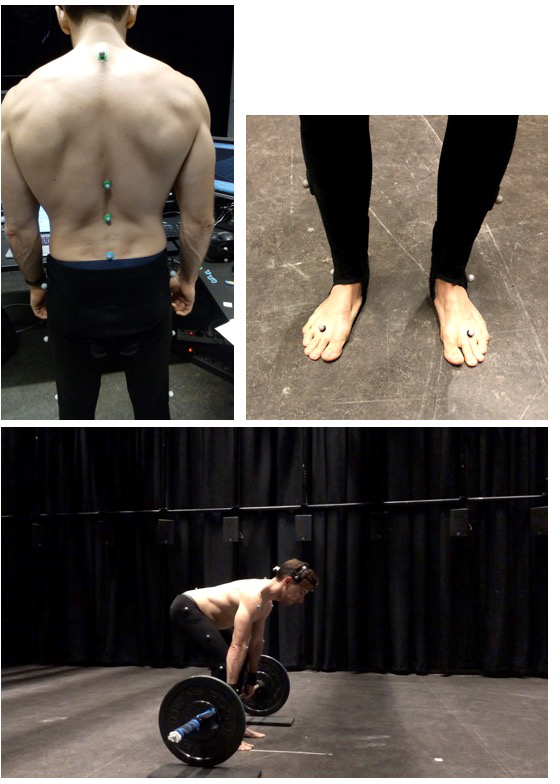
\includegraphics[width=.8\textwidth]{figures/combination_markers.jpg}
\caption{Mocap markers positioning}
\label{fig:set-up}      
\end{figure}

A schematic representation of quantities that were used as experimental parameter are shown in Fig. \ref{fig:sketch_quantities}.
\begin{description}
\item[Spine bend] The sum of the consecutive distances between spine markers ($$spine dist = d0+d1+d2$$) 
\item[B-F distance] The planar distance between the line connecting the extremities of the barbell and the markers on the front part of the foot. The smaller of the two distances was considered.
\end{description}

\begin{figure}[!h]
\center
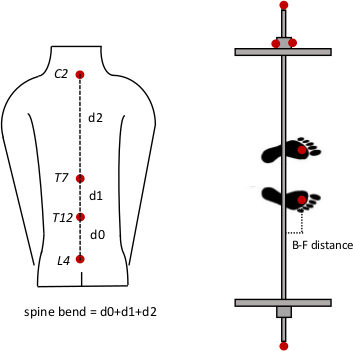
\includegraphics[width=.8\textwidth]{figures/Sketch_spine_final.jpg}
\caption{Mocap markers positioning}
\label{fig:sketch_quantities}      
\end{figure}


Mocap recordings were performed on a dedicated Windows computer. The system evaluated the 3D markers positions at a frequency of 100 Hz. These position were transmitted in real-time as OSC message to Max from Cycling UDP receiver implemented in Max4Live, as audio effect within Ableton Live\textsuperscript{\textregistered} . The Max4Live patch was responsible for starting and stopping the music, providing the sonification based on the physical parameters and storing the data.

A picture of the interface is provided in Fig \ref{fig:interface}
\begin{figure}[!h]
\center
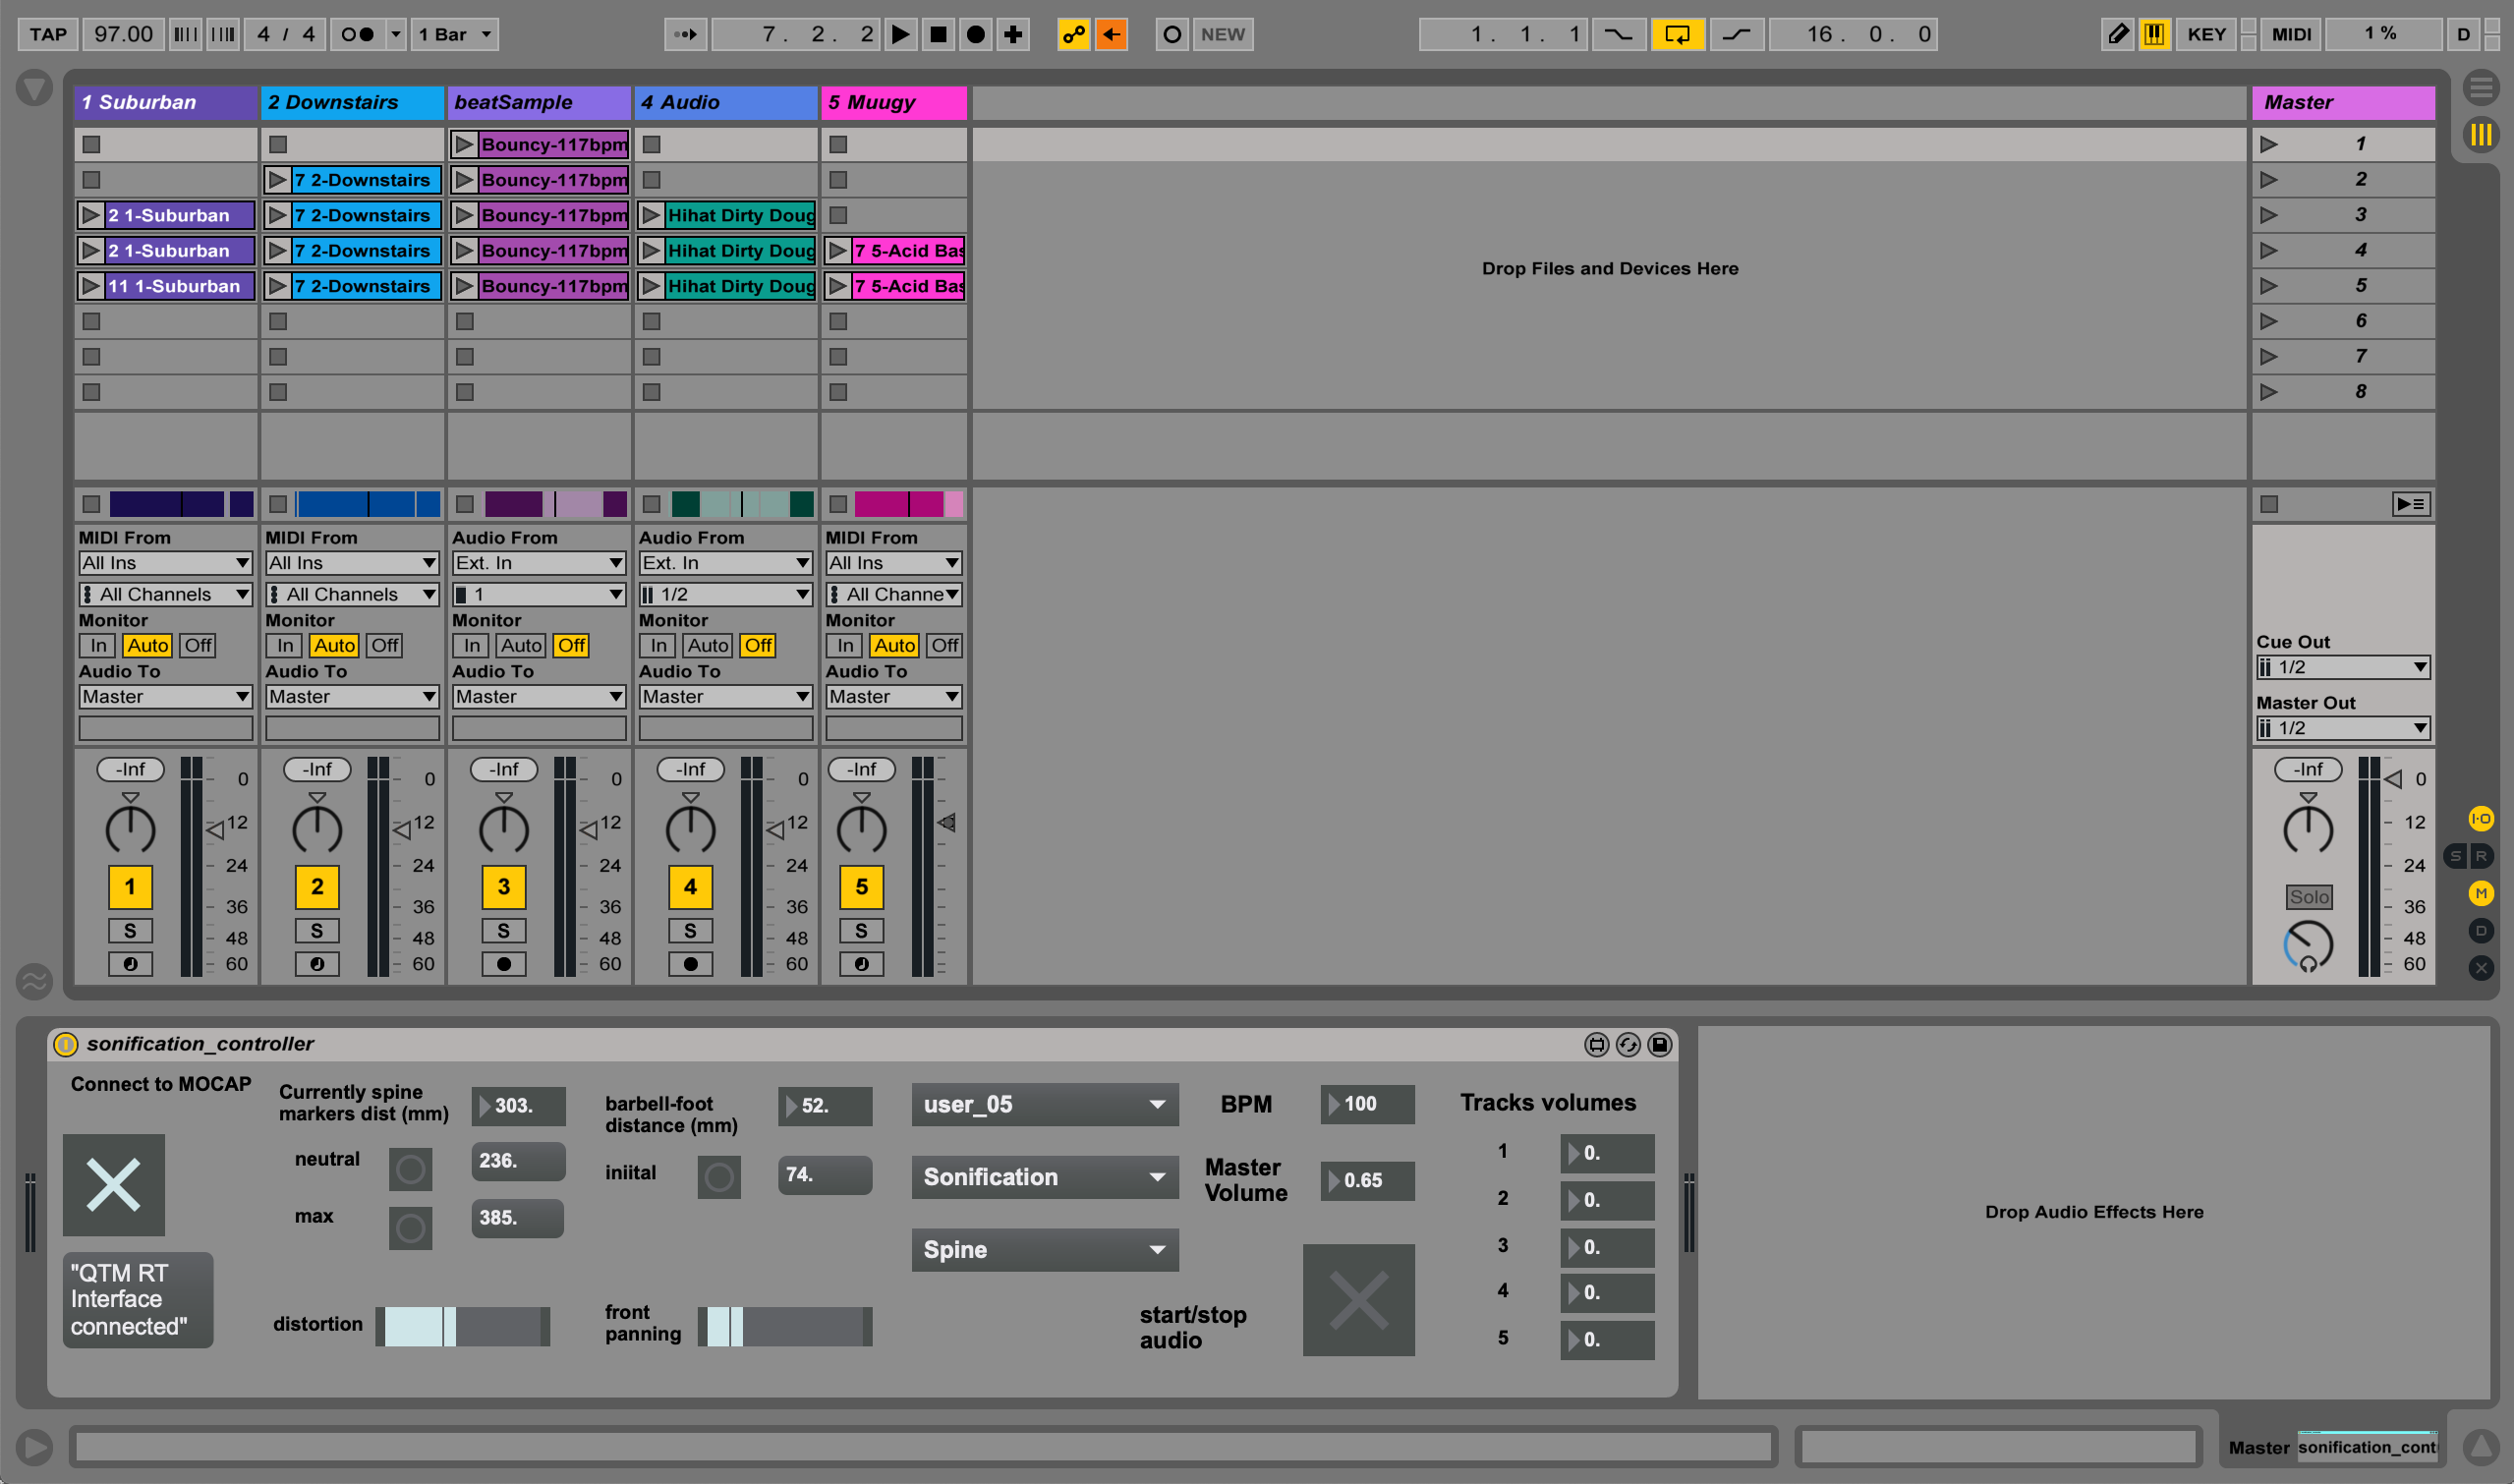
\includegraphics[width=.6\textwidth]{figures/interface.png}
\caption{Interface of console computer running Ableton Live with house developed MAX4Live controller effect}
\label{fig:interface}      
\end{figure}


\subsection*{Experimental procedure}
Once in the lab, participants received a description of the experiment. They were asked to sign an informed consent form and fill in a questionnaire with general information: gender, age, level of experience with weightlifting, music education, injuries. After that, a video was shown of an expert performing 10 deadlifts, in front and side view.
Participants were then equipped with the markers set-up. The Qualisys software made used of a pre-trained skeleton model to recognize the body parts across different subjects. The correct markers labelling was checked at this stage. 
One of the authors is certified Level 2 crossfit trainer and functioned as instructor during the experiments. A warm-up routine was provided by the instructor to all participants prior to the tests.

Before starting performing deadlift, reference parameters for each subject were recorded, specifically:
\begin{description}
\item[Neutral spine] Participants were asked to grab the bar and keep spine in unloaded position.
\item[Max spine bend] Participants were asked to grab the bar and slightly bend forward. The instructor was helping them finding this position letting them bend the spine  up to incorrect but stil not dangerous position
\item[Initial barbell-foot distance] Participants were asked to grab the barbell on the ground as they would start the movement and they were instructed that the barbell needed to be approximately in the middle of the foot
\end{description}

The actual tests started with a serie of 10 deadlifts at own tempo, middle-low pace. This was taken as control condition for the analysis. Afterwards participants were randomly split in two groups, as homogeneous as possible in terms of gender, experience level and age (see sketch in Fig. \ref{fig:workflow}).
\begin{figure}[!h]
\center
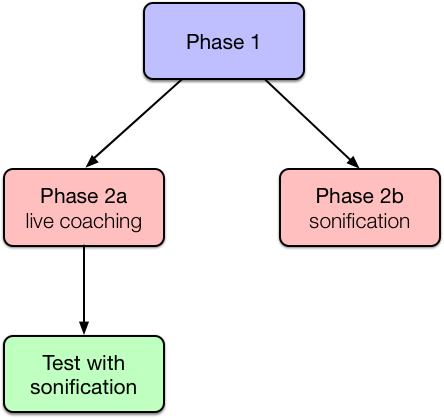
\includegraphics[width=.5\textwidth]{figures/Experiment-flow.png}
\caption{Scheme of the experiment design protocol}
\label{fig:exp-flow}      
\end{figure}

One group of participants received verbal feedback by the instructor the other group received sonification as feedback. The groups are hereafter called \emph{instructions group} and \emph{sonification group}.

Participants of both groups were asked to perform 10 deadlifts for each of the following Points of Performance, in randomized order:
\emph{Spine},\emph{Barbell} and \emph{Combination}

The test leaders informed the participant to only focus on the specific point of performance and that continuous feedback (either as verbal instructions or as sonification) would have been given if the movement was deviating from correctness.

The provided feedbacks corresponded to, respectively for the \emph{instruction group} and the \emph{sonification group} and for the specific point of performance:

\paragraph{Instructions feedback} 
\begin{description}
\item  \emph{Spine}: You
\item  \emph{Barbell}: sonification 
\item  \emph{Combination}: a tempo synchronization condition based on the initial SPM of the runner
\end{description}


\paragraph{Sonification feedback}
\paragraph{Instructions feedback} 
\begin{description}
\item  \emph{Spine}: sonification based on the spine curvature only, 
\item  \emph{Barbell}: sonification 
\item  \emph{Combination}: a tempo synchronization condition based on the initial SPM of the runner
\end{description}




%Do you practice any sports?
%If yes, how often per week?
%Do you have experience with weight lifting functional movements (deadlift, airsquat, snatch)? 
%If yes, for how long?
%Do you work-out with or without music?
%As what kind of learner do you perceive yourself?
%Have you ever had musical training?
%If yes, how long (in years)?
%If yes, at what age did you start?
%Do you currently play an instrument?
%Do you have normal (or corrected to normal) vision?
%Do you have normal (or corrected to normal) hearing?
%Do you suffer from tinnitus?
%Did you suffer any injuries within the last 6 months?
%If yes, what were they?
%
%
%

After each serie of repetitions, a break of 5 minutes was introduced to enable the participant to recover sufficiently. During the break they were asked to fill out a Rating of Perceived Exertion (RPE) questionnaire \cite{borg1998borg} and indicate how heavy the effort had been during the exercise, ranging from 6 ("no exertion at all") to 20 ("maximal exertion"). 
In addition, they rated the level of physical enjoyment of the previous run on the 8-item version of the Physical Activity Enjoyment Scale (PACES) \cite{kendzierski1991physical}, a single factor scale to assess the level of enjoyment during a physical activity in adults across exercise modalities.
In order to test the motivational properties of the feedback, participants also performed a modified version of the Brunel Music Rating Inventory 2 (BMRI-2) test \cite{karageorghis2006redesign}. In this test, they were asked to rate on a 7-point Likert scale: clarity, pleasantness, accuracy, motivational properties and usability of the presented audio feedback. % Furthermore they were asked if they would use such a system to guide them to optimal movement technique
All questionnaires were implemented as Google forms on a dedicated computer within the same room.

 

\subsection*{Stimuli}

In all conditions the same music piece was played. The piece was specifically composed for this experiment by the authors. The music was composed respecting the following requirements:
\begin{itemize}
\item to be unknown, to avoid personal affection
\item to be instrumental (no lyrics), to avoid focus on content
\item to have a clear beat, in order to stimulate repetitive movements.
\end{itemize}

For the sonification feedback 
the spine spine curvature
ithe music was distorted using the degrade object implemented in MAX/MSP, proportionally to the detected movement error.

\subsection*{Data acquisition}

The markers positions in the 

The markers positions were continuously transmitted as OSC to an in-house MAX/MSP program running on the same tablet, which implemented the synchronization strategies and provided the audio. Data were collected every 10 milliseconds and stored as .txt. file on the control computer





\subsection*{Data analysis}

A preliminary analysis of normality of the data 

t-test 


speak of power as the probability of not making a beta, or a "Type II" error, which refers to falsely concluding that there was no difference (e.g., between experimental and control groups) when in fact there was a difference, but the study failed to show it.

\section*{Results} \label{sec:results}



\subsection*{Differences in performance between feedbacks}


\paragraph{Spine bend differences}

\begin{figure}[!h]
\center
  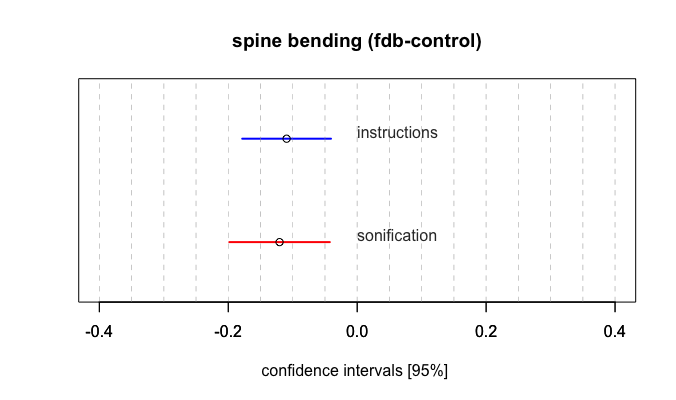
\includegraphics[width=.5\textwidth]{figures/CI_spine_bending.png} 
  \caption{Differences between the instruction and sonification feedbacks} 
  \label{fig:boxplot}      
\end{figure}


\begin{figure}[!ht] 
    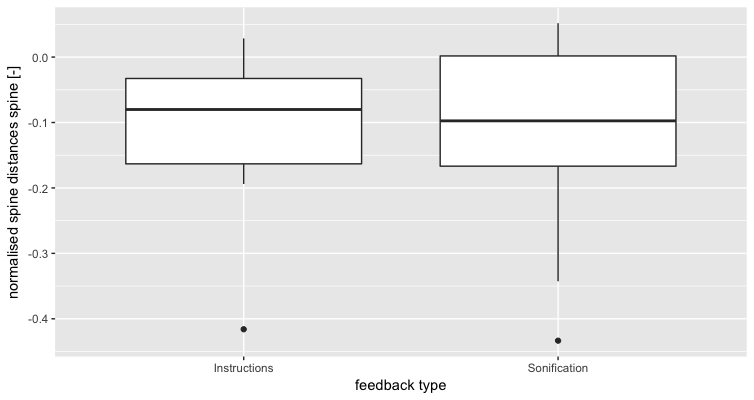
\includegraphics[width=.45\textwidth]{figures/boxplot.png}
\caption{boxplot between 2 feedbaccks}
\label{fig:boxplot} 
\end{figure}


\paragraph{Barbell horizontal displacement}

%% OLD TABLE






%\begin{table}[!ht]
%%\begin{adjustwidth}{-2.25in}{0in} % Comment out/remove adjustwidth environment if table fits in text column.
%\centering
%\caption{
%{\bf Table caption Nulla mi mi, venenatis sed ipsum varius, volutpat euismod diam.}}
%\begin{tabular}{|clclc|clc|c|}
%\hline
%\multicolumn{1}{|c}{\bf Feedback type} & \multicolumn{6}{|c|}{\bf Point of Performance}\\ \hline
%\multicolumn{1}{|c|}{\bf} & \multicolumn{2}{|c|}{\bf Spine bend}& \multicolumn{2}{|c|}{\bf Barbell distance} & \multicolumn{2}{|c|}{\bf Combination}\\ \hline
%
%$Instructions $  & cell2  & cell3& row 1 & cell5 & cell6& cell6 \\ \hline
%$Sonification $  & cell2 & cell3  & row 2 & cell5  & cell6 & cell6 \\ \hline
%
%\end{tabular}
%
%\label{table1}
%%\end{adjustwidth}
%\end{table}
%

% Table generated by Excel2LaTeX from sheet 'tablePaper'
\begin{table}[!h]
  \centering
  \caption{Comaprison of }
    \begin{tabular}{|l|r|r|r|r|r|r|}
    \hline
          & \multicolumn{6}{c|}{\bf Point of Performance} \\
   \hline
          & \multicolumn{2}{c|}{\bf Spine bend} & \multicolumn{2}{c|}{ \bf Barbell distance} & \multicolumn{2}{c|}{\bf Combination} \\
     \hline
   \bf Feedback type & \multicolumn{1}{l|}{mean} & \multicolumn{1}{l|}{sd} & \multicolumn{1}{l|}{mean} & \multicolumn{1}{l|}{sd} & \multicolumn{1}{l|}{mean} & \multicolumn{1}{l|}{sd} \\
    \hline
    Instructions &       &       &       &       &       &  \\
    \hline
    Sonification &       &       &       &       &       &  \\
     \hline
    \end{tabular}%
  \label{tab:addlabel}%
\end{table}%





\subsection*{Pairwise differences}



A KS-test for normality revealed that g differences for Adaptive sync condition were normally distributed ($p=0.06$) as well as for the  Plus 30\% ($p=0.2$). The conditions Initial sync ($p=0.022$), Minus 30\% ($p=0.016$) and No music ($p=0.001$) were not normally distributed. 
Paired t-tests were performed on the normally distributed pairs, Wilcoxon tests on the non-normally distributed ones. A summary of the results is shown in Table \ref{tab:parwise} with effect size Cohen $d$ for t-tests and Pearson correlation coefficient $r$ for Wilcoxon tests:




\subsection*{Questionnaires information}

Participants were asked to rate pleasantness and motivational effect of the different synchronisation strategies on a 7-point Likert scale. No overall significant difference was found across conditions using a non parametric Friedman test ($p > 0.05$). 

When comparing independent groups by means of Mann Whitney tests, differences in pleasantness ratings were observed between participants with music education (17) and participants without music education (11) for some of the experimental conditions.
The results are presented in Table \ref{tab:table1}.
%Ratings for each condition were compared among independent groups: participants with music education and participants without by means of Mann Whitney tests.



No significant differences were found across gender and across training level of participants. 

\section*{Discussion} \label{sec:discussion}

In this case no effect of arousal produced by the acoustic stimulus was noticed compared to the no sonification condition. E certo se era distorsion!!




Portability of the system could be improved by adoption of current systems for back posture detection ViPerform tm Assessment Modules


Our hypothesis was is that such system could be comparable to the verbal instructions by and instructor in terms of performnces 

Fritz \emph{et al.}  \cite{fritz2013musical}  distortion linked to agency positive feedback?


However no significant differences were found between the two feedbackss across participants in terms of pleasantness and motivational qualities: reasons could be

choice of music (elaborate)
people used to having a coach
people prefer human feedback

From Tate (2010) NO RETAINING TESTS in his study nor in present experiment
 Each biofeedback method appeared to result in moderate to large treatment effects immediately after treatment. However, it is unknown whether the effects were maintained. Future studies should ensure adequate randomization of participants and implementation of motor learning concepts and should include retention testing to assess the long-term success of biofeedback and outcome measures capable of demonstrating coordinative changes in gait and improvement in function.

Extend conversation to WELL-BEING also for PhD thesis



%The design of sonification strategies has been largely investigated for runners gait parameters modifications \cite{bank2011comparing}

\subsection*{Conclusions}

An experiment was performed to check the influence of different music synchronisation strategies on runner's foot strike impact. From the analysis, synchronisation seems not to lead to variations in impact level. However, music onset seems to cause an average impact level increase of 17\% compared to running without music, irrespective of the synchronisation strategy.
No significant difference in pleasantness and motivational effect were observed across the different synchronisation strategies, although phase alignment of the footfalls with music beats seems to be preferred by people with musical background. 



\section*{Acknowledgments}
The authors would like to thank the students of the course Sysmus2017 for the help carrying out the experiments. Bruno De Wannemaeker and the staff of the Topsport Hall in Gent is also gratefully acknowledged for their availability and support during the tests.
\nolinenumbers

%\section*{References}
% Either type in your references using
% \begin{thebibliography}{}
% \bibitem
% Text
% \end{thebibliography}
%
% OR
%
% Compile your BiBTeX database using our plos2015.bst
% style file and paste the contents of your .bbl file
% here.
% 

\bibliographystyle{plos2015}
\bibliography{/Users/valerioipem/Dropbox/MyIPEM/Publications/IPEMBibliography}




\end{document}


